\chapter{Case Study: A Privacy-preserving Video Doorbell}
\label{sec:case_study}
This chapter presents a case study that focuses on the design and implementation of a specific type of IoT device - an Internet-enabled video doorbell using our privacy-preserving framework. We assume the communication model to be the user-to-IoT model, that is, the IoT device (video doorbell) is located in the user’s home network and communicates (potentially indirectly) with the end-user device (smartphone). The goal of this case-study is to support a feature-rich IoT offering while providing strong security and privacy properties.

\section{Features and system design}
In addition to the security guarantees described in the last chapter, video doorbell systems have unique features. Here, we present the details of our design.

\subsection{Features}
We consider there should be five prominent use cases in the system:
\begin{itemize}
	\item \textbf{Registration.} The user should be able to register a mobile device to the doorbell. Only trusted devices can access the data and manage settings.
	\item \textbf{Video streaming.} The user with a registered device should be able to access video captured by the camera at any time they wish.
	\item \textbf{Face detection and push notification.} Whenever a visitor appears in front of the camera and/or presses the physical doorbell button, all users registered to the doorbell should receive a push notification message on their smartphones.
	\item \textbf{Setting management.} The user should be able to manage settings, including changing face detection threshold, recording voice to be played, removing trusted devices, etc.
	\item \textbf{Two-way conversations.} The system should enable two-way conversations, in which the visitor can directly speak to the doorbell user and the user can play pre-recorded voice in response. The pre-recorded voice acts as an alternative way of answering to decrease the high latency introduced by Tor.
\end{itemize}

\textit{Fig. \ref{fig:usecase}} shows the use case diagram of the system.

We describe the specifics of our implementation in more detail below. At a high-level, our video doorbell consists of a computing platform (Raspberry Pi), a video camera and an external sound card.

\begin{figure}
	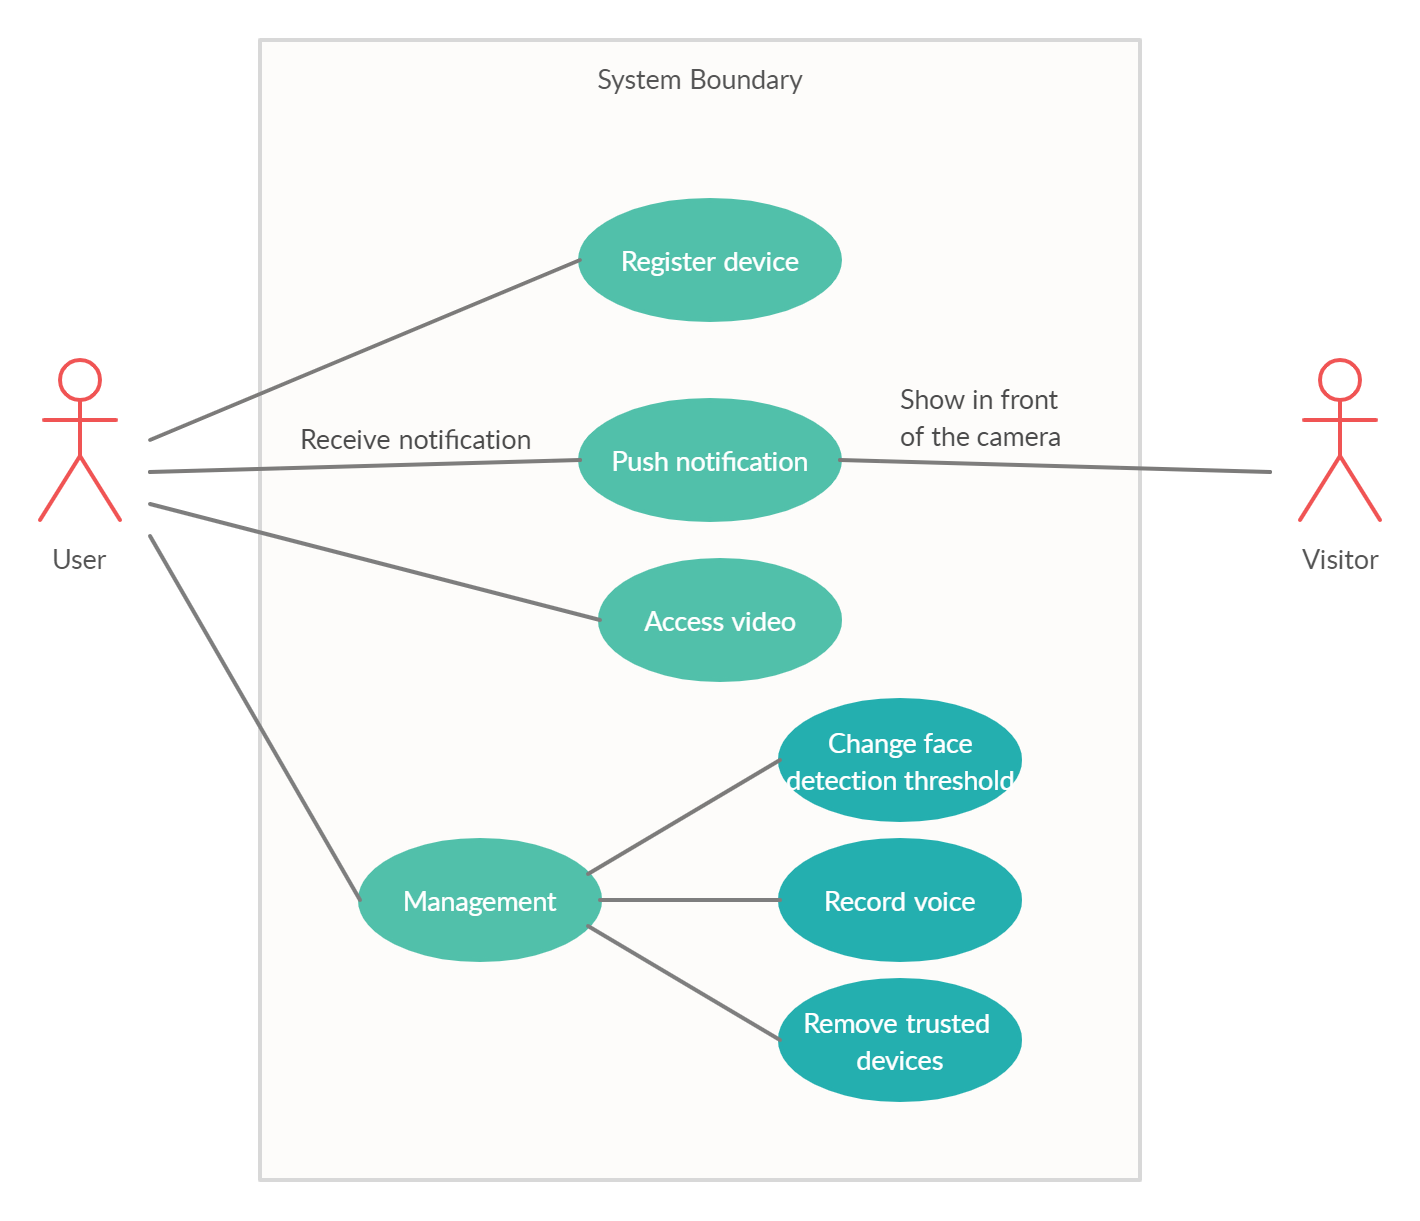
\includegraphics[width=\linewidth]{Use_case_diagram.png}
	\caption{Use case diagram}
	\label{fig:usecase}
\end{figure}

\subsection{Network architecture}
\label{sec:netarch}
\textit{Fig. \ref{fig:architecture}} shows the network architecture of the system. Both the client and server communicate using Tor to prevent an adversary from trivially identifying the devices' traffic. Additionally, we configure Tor on the doorbell side to use the Snowflake pluggable transport. Snowflake is an add-on for Tor that tunnels Tor traffic through WebRTC \cite{macmillan2020evaluating}, a protocol that is popular for videoconferencing (e.g. Google's Hangouts or Jitsi). By using Snowflake, an adversary that monitors the communication from the user's home cannot easily identify the use or presence of the IoT doorbell, since its traffic is disguised as WebRTC flows.

\begin{figure}
	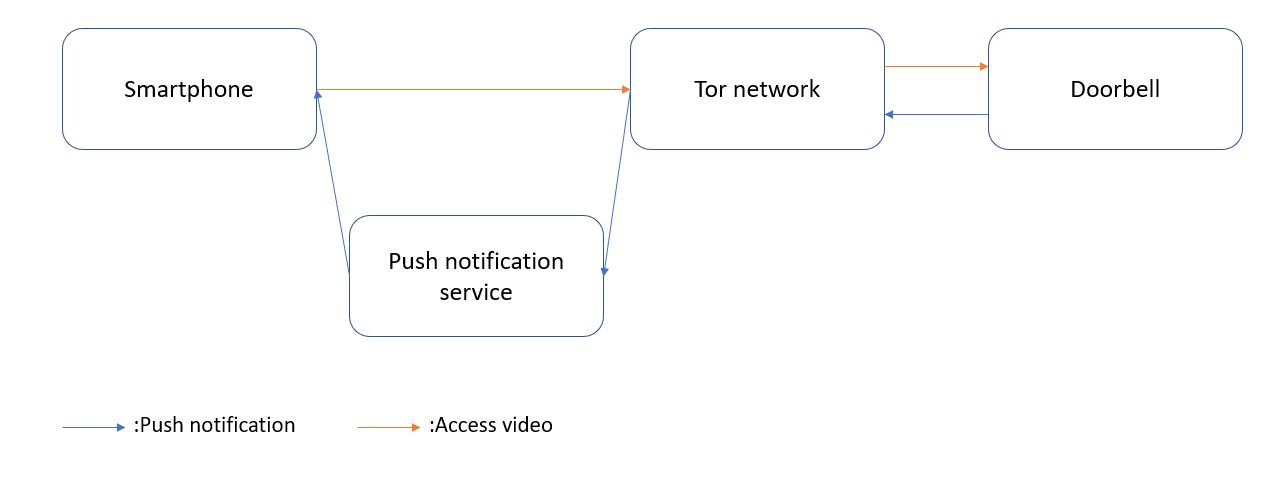
\includegraphics[width=\linewidth]{architecture.png}
	\caption{Network architecture diagram}
	\label{fig:architecture}
\end{figure}

\subsection{Operation}

\textbf{Registration.} The very first stage of using the system is the registration process. To have their devices registered on the doorbell, the users should first connect to the same wireless network with the doorbell. Then the app should allow the user to register easily by searching the doorbell using mDNS (Multicast DNS, also known as mDNS, is a protocol that resolves hostnames to IP addresses in small networks, like local home networks, which do not include a local name server.). During the registration process, the smartphone app performs a key exchange with the doorbell and receives randomly generated credentials for the user to set up in Tor. We use Orbot, an open-source implementation of Tor, on the smartphone. Currently, our implementation supports Android, although providing support for iOS should be straightforward.

\textbf{Playing video and authentication.} Our IoT doorbell allows the user to observe activities that occur at their doorstep by activating the doorbell's video camera and streaming the video to the smartphone app. As soon as the user presses the PLAY button in the app, it will work with Orbot and send an RTMP PLAY request to the video server running on the doorbell. The video server will then forward an authentication request (in the form of an HTTP GET request) to the authentication server (running on another port on the doorbell). The server should serve video to the user through Tor if the authentication succeeds (i.e., the app is registered and has not been revoked) and shut down the connection otherwise.
\textit{Fig. \ref{fig:playvideo}} shows the flow of playing video and authentication. As described above, there are five components in the flow: the user (\textit{user}), the smartphone app (\textit{app}), the Orbot app (\textit{Orbot}), the video server (\textit{videoserver}) and the authentication server (\textit{authserver}).

\textbf{Face detection, push notification, and answering the door.} The doorbell constantly detects if there is a human face appearing in front of the camera. Whenever a visitor appears, the system should send a notification to the user's devices through Google's push notification service, Firebase Cloud Messaging (FCM).

By clicking on the notification message on her phone, the user should be able to access the video immediately and choose to play pre-recorded audio on the doorbell device to the visitor.
\textit{Fig. \ref{fig:push}} shows the flow of face detection, push notification, and answering the door.


\begin{figure}
	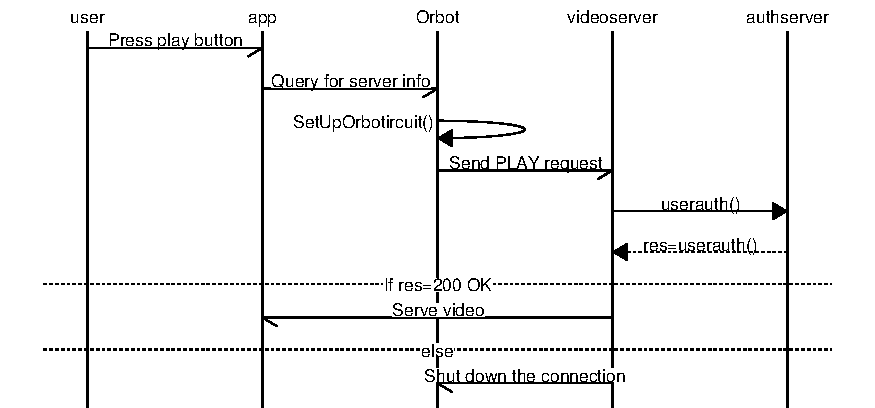
\includegraphics[width=\linewidth]{Sequence_diagram_playvideo.pdf}
	\caption{Sequence diagram: Video streaming}
	\label{fig:playvideo}
\end{figure}
\begin{figure}
	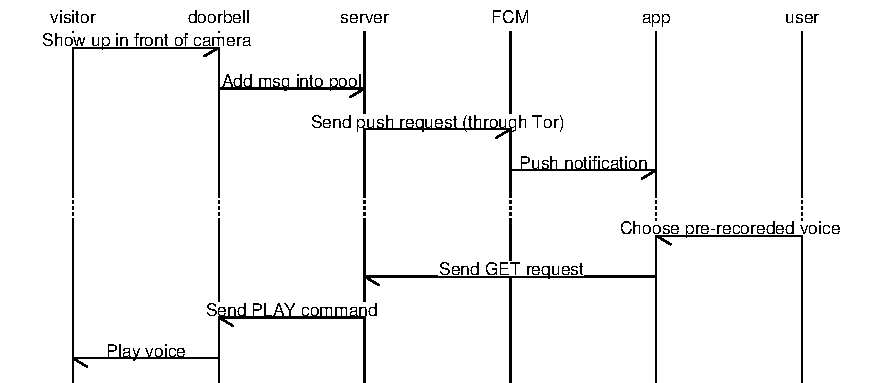
\includegraphics[width=\linewidth]{Sequence_diagram_push.pdf}
	\caption{Sequence diagram: Push notification}
	\label{fig:push}
\end{figure}


\section{Face detection}
A core feature of our privacy-preserving IoT framework is the avoidance of points of centralization. Although many cloud-based face detection services exist (e.g., Google's Firebase MLKit), we restrict our IoT doorbell to use on-device face detection. (We also remark that our devices do not perform face \textit{recognition}, which is a seperate task that attempts to identify the individual who the face belongs to.) 

For the face detection task, we use the pre-trained CascadeClassifier \cite{viola2001rapid}. Cascade Classifiers based on Haar-like features were introduced in 2001 and are still widely used in face detection \cite{sharifara2014general}. Pre-trained Cascade Classifiers have a short execution time and small calculation load, making them a good choice for on-device calculations on IoT devices with low computational power.

We sample 6 frames per second in the actual implementation, transform them into gray-scale images, and feed them to the pre-trained classifiers. The detector is disabled for 5 seconds (which also matches the push notification interval) after a successful detection to prevent abusing resources. 

\section{Device specifications}
We configured a RaspberryPi 4 model B as the doorbell device. The RaspberryPi 4 has a built-in Wi-Fi antenna, and we combined the device with a camera module and external sound card. The RaspberryPi ran the Raspbian Jessie OS, which is a version of Debian Linux optimized for the RaspberryPi platform.

The RaspberryPi 4 model is equipped with  2GB of RAM and a 4-core CPU of 1.5 GHz, which provides sufficient computation power for our requirements.

\section{Push notification}
As with other IoT doorbell systems, our implementation alerts the user whenever an individual approaches their house. To notify the user whenever a visitor is present in front of the camera, the system adopts Google's Firebase Messaging Service.

We designed two types of messages: \textbf{BELL} (sent when someone pushes the doorbell device’s physical button) and \textbf{DOOR} (sent when someone comes in front of the camera). The packet includes a message (including the type mentioned above), a timestamp, and the user's instance token. The message and timestamp are encrypted using AES-256-GCM with pre-shared keys (which are shared in the registration process described later).

In order to prevent the third-party service provider (i.e., Google) from obtaining sensitive information (e.g., the comings and goings of visitors) by analyzing timing information, we further cover the traffic using another message type \textbf{DUMMY}, and send messages in a fixed interval of 5 seconds. The dummy packets have very similar structures to the normal ones, but have different types to be recognized by the client app. We note that \textbf{BELL}, \textbf{DOOR} and \textbf{DUMMY} packets are all encrypted and appear indistinguishable to the push service provider. We ensure that the system sends a packet every 5 seconds. However, it is worth mentioning that there may be potential optimizations on both the traffic cover mechanism and the push notification system. We will discuss them in Section \ref{sec:traffic_cover} and \ref{sec:decentralized_push}, and show a simple proof-of-concept of a fully-decentralized push notification system.




\section{Video streaming}
The doorbell device captures video using the RaspberryPi's camera module and audio through an external sound card. The video captured is encoded and served in flv format through HTTP. We chose to encode the videos in flv format because flv support is common in many operating systems and thus support future portability to other platforms.

Our system adopts two layers of authentication on top of video streaming. The first layer of authentication is \textit{onion authentication}. Provided along with Tor, it requires the user to have specific credentials set up in their Tor (Orbot) client. The onion host refuses to connect if the client does not have such credentials. The second layer of authentication is the \textit{RTMP authentication}. In order to access the video, the user will have to add credential arguments in addition to their RTMP PLAY request. \textit{Fig. \ref{fig:url}} shows the components of the video serving URL. In the URL, \textit{appname} and \textit{streamname} are Nginx settings and of the user's choice. \textit{usertoken} is a random number securely generated from the client app (upon the first launch), and the following equation calculates userpassword:

\[
userpassword = HMAC(seed, usertoken)
\]

where the HMAC is based on SHA256.

The server checks if \textit{all} credentials match and shuts down the connection if any are incorrect. The \textit{seed} is a per-device secret, and its generation and use is explained in more detail in Section \ref{sec:registration}.

\begin{figure}
	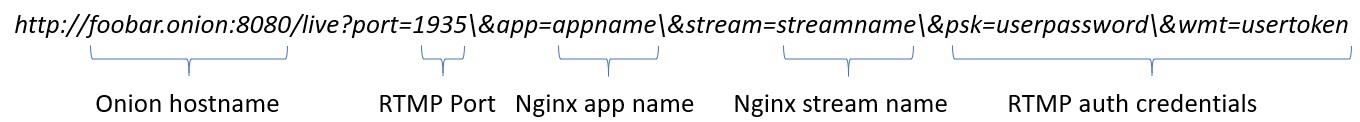
\includegraphics[width=\linewidth]{fig_url.jpg}
	\caption{An example of video serving URL}
	\label{fig:url}
\end{figure}



\section{Android App}
We implemented an Android App to pair with the video doorbell service. The app runs on the end-user smartphone device and grants users access to the doorbell device and data. The app has the following primary functions:

\subsection{Registration} 
\label{sec:registration}
For registration, the client sends JSON-formatted data in an HTTP POST request to port 8080 of the server (running on the doorbell device). This occurs over WiFi in the user's home. The server will then respond with another JSON-formatted data, including the seed (randomly generated 16-bit integer) for calculating the secret keys, the onion hostname for accessing the video service, and the onion authentication cookie. The app will then automatically send a configuration string (including the authentication cookie) required by Orbot to the user’s clipboard for her to set up the service quickly. 

\textit{Fig. \ref{fig:app_sc}} shows the main (registration) GUI of the app.


\subsection{Media player} The app has the VLC player integrated for video streaming. This allows users to see what is occurring at their doorstep. Working with Orbot, the media player streams the video through the onion network, which prevents adversaries from eavesdropping on the transmitted video. The use of Snowflake (as described in Section \ref{sec:netarch}) also disguises the video stream.

\subsection{Two-way communication}
The media player streams both video and audio and thus enables the user to see and hear visitors. Meanwhile, the user has the option to play pre-recorded voice samples (which can be managed through the app as well, as described in Section \ref{sec:management}) to communicate with visitors. We envision supporting real-time two-way communication as a future feature.

\subsection{Device management}
\label{sec:management}
The doorbell serves a webpage for the user to manipulate device settings, including changing the face detection threshold, revoking authentications, recording voice, etc. The management page is only accessible in the local network (that is, the user's smartphone device must be in the same wireless network as the doorbell device to manipulate settings) and requires a password for access.

\textit{Fig. \ref{fig:app_sc}} shows the entry page, the preference page, and the token management (where user can revoke trusted devices) of the app.

\begin{figure}
	\begin{minipage}[t]{0.3\linewidth}
		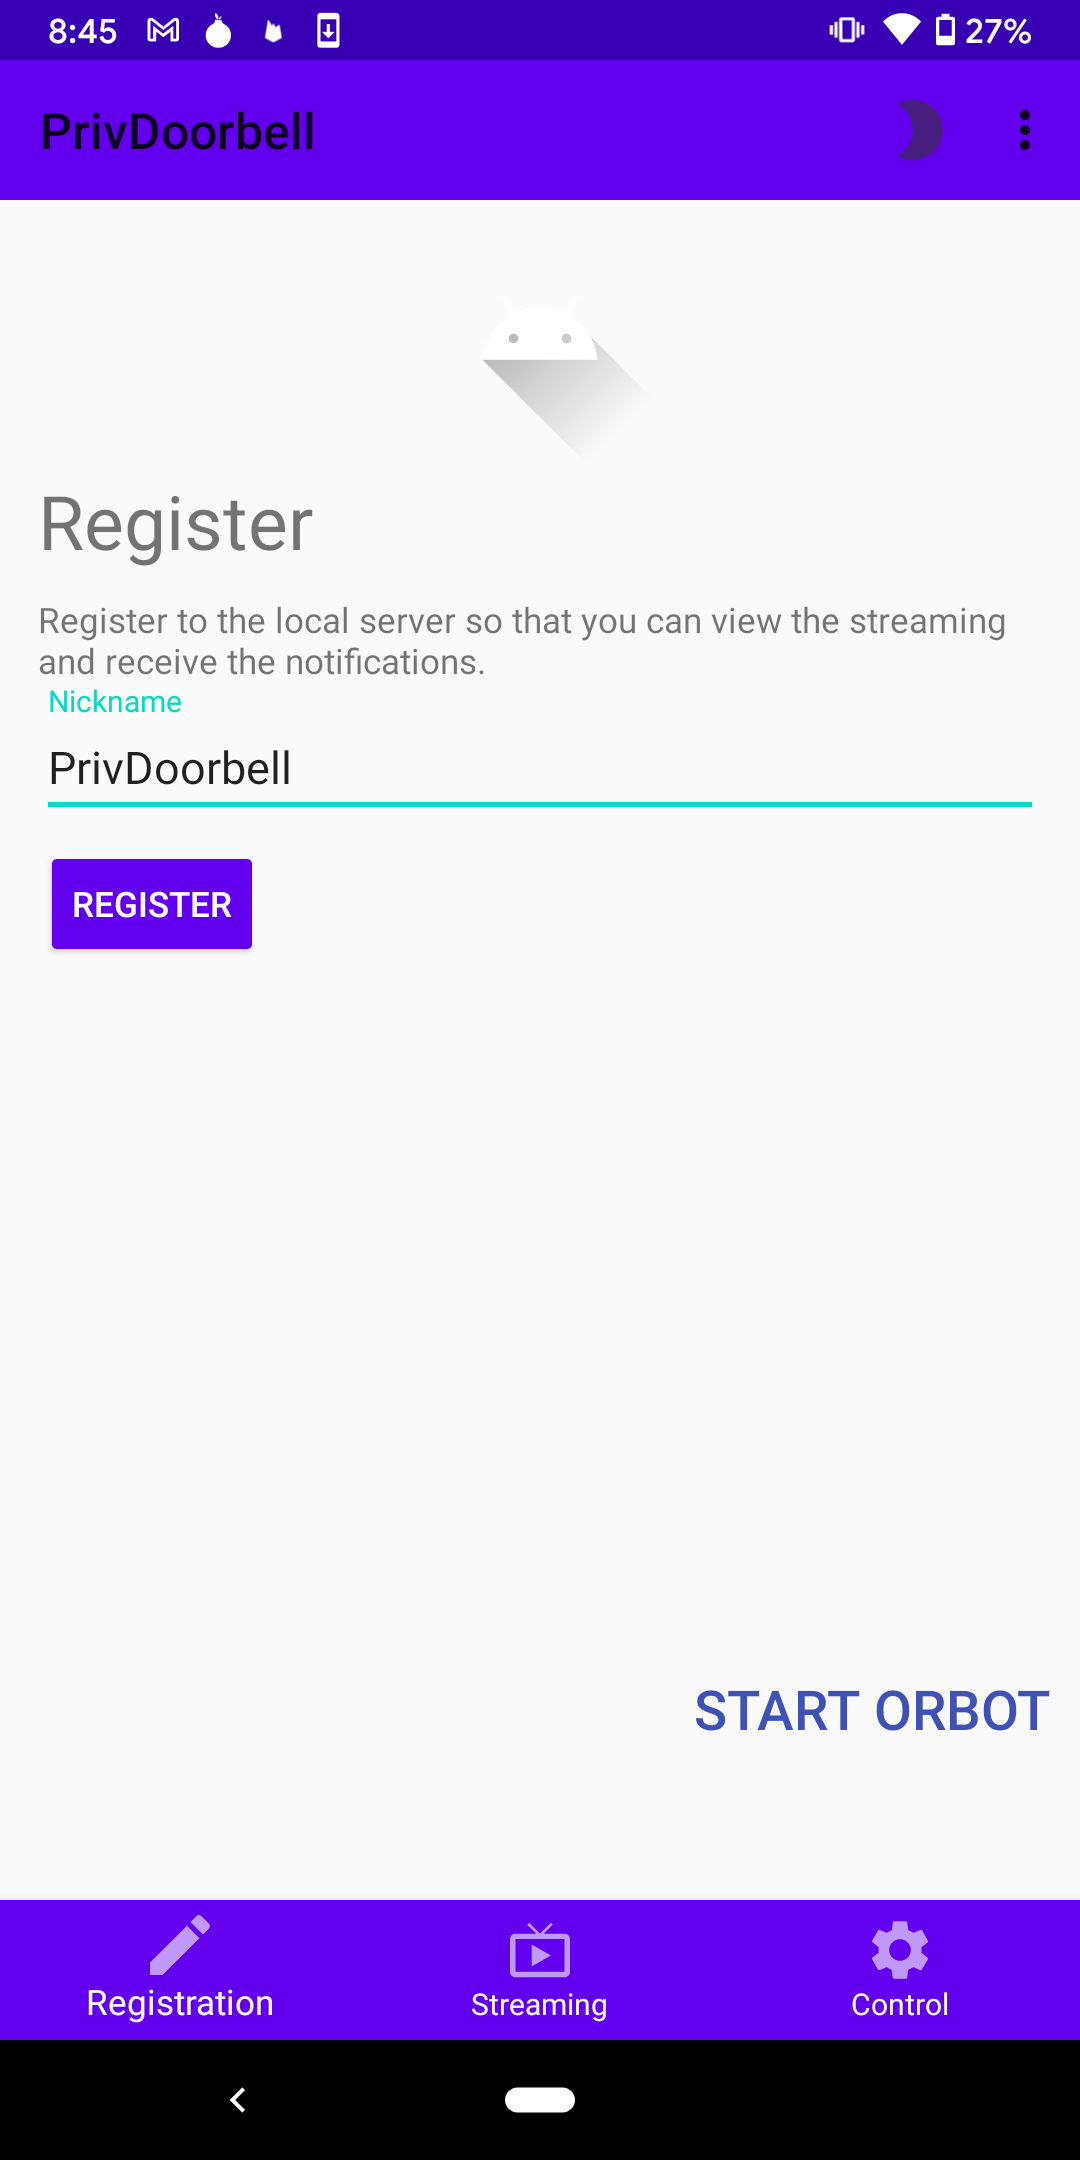
\includegraphics[width=\linewidth]{app_sc_main.png}
	\end{minipage}
	\begin{minipage}[t]{0.3\linewidth}
		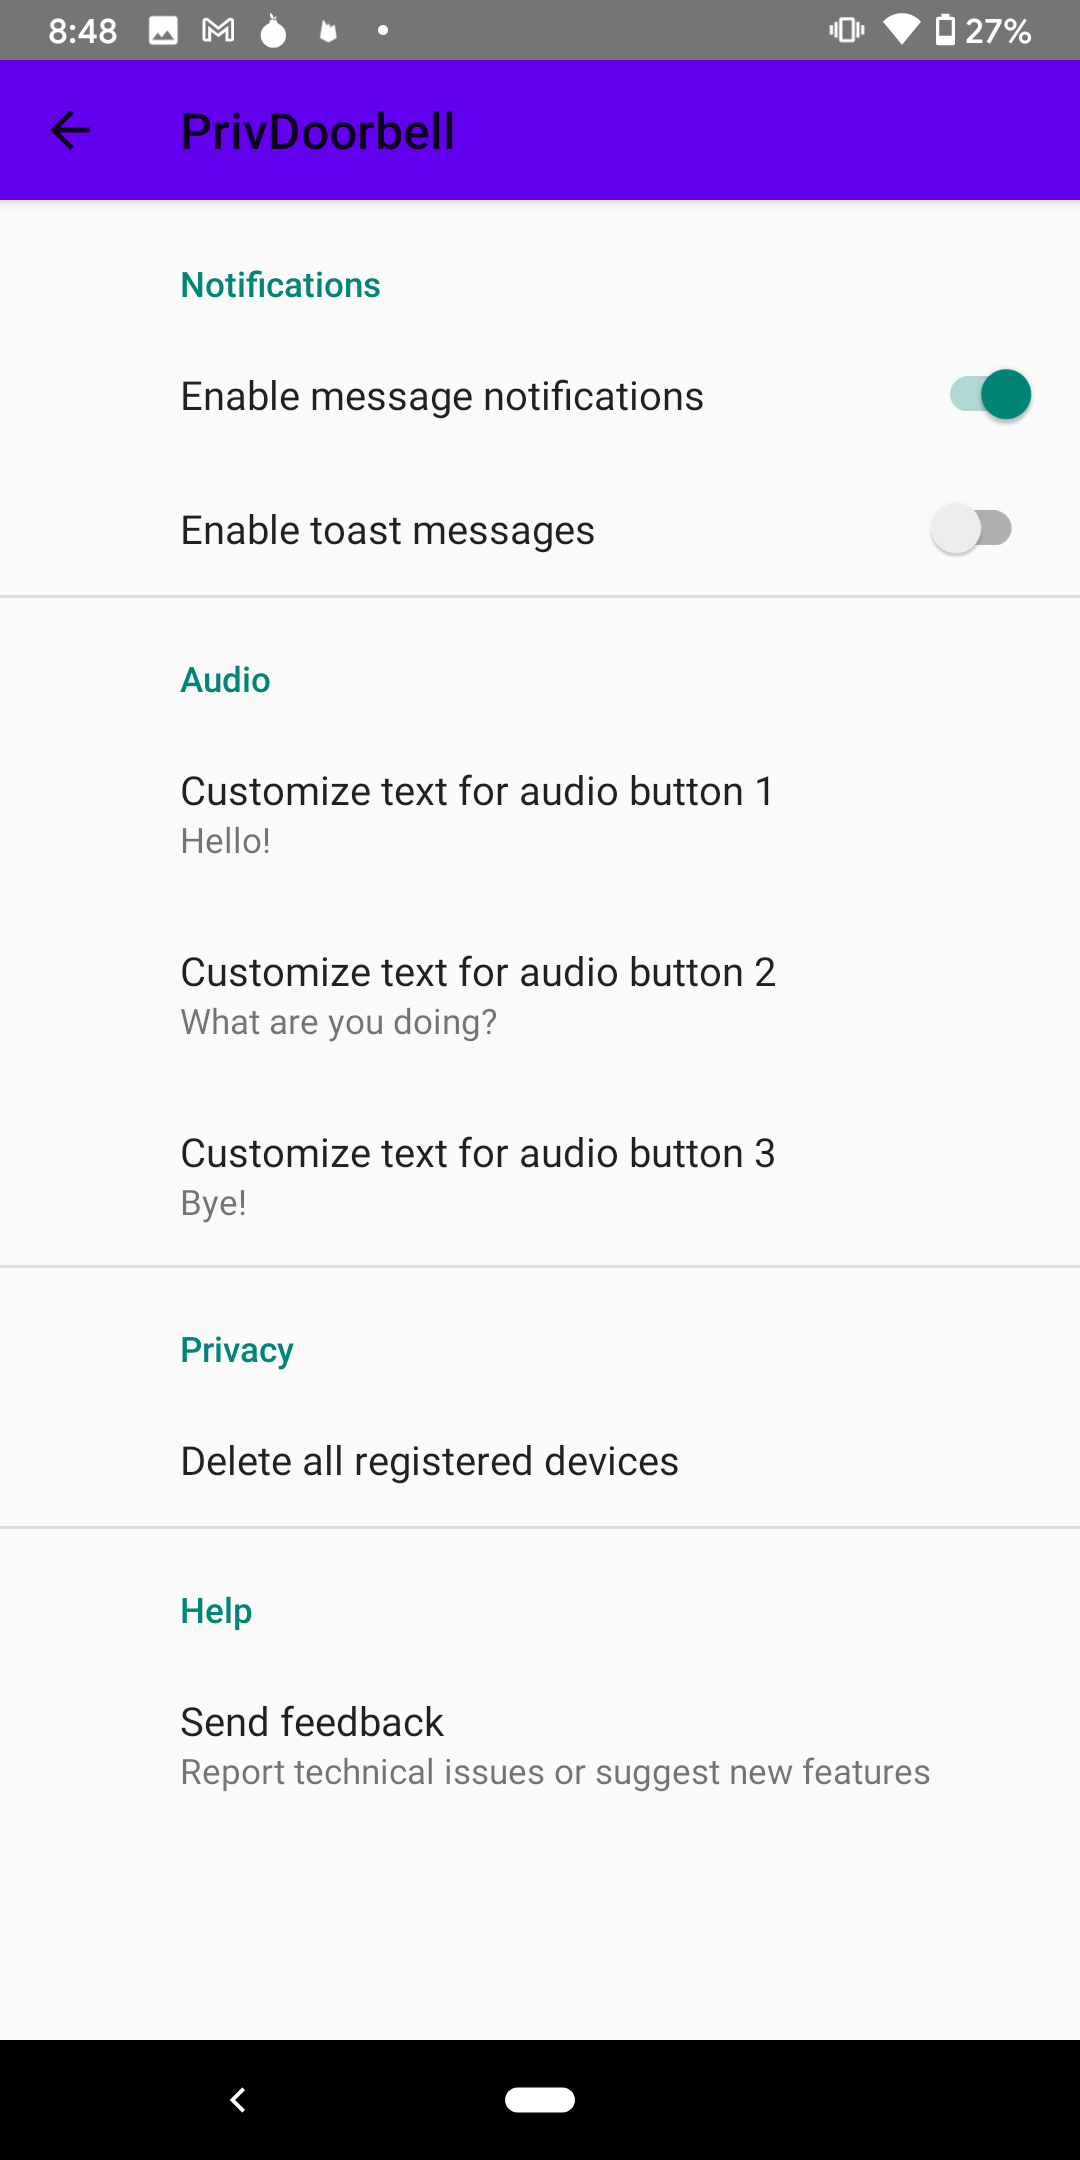
\includegraphics[width=\linewidth]{app_sc_management.png}
	\end{minipage}
	\begin{minipage}[t]{0.3\linewidth}
		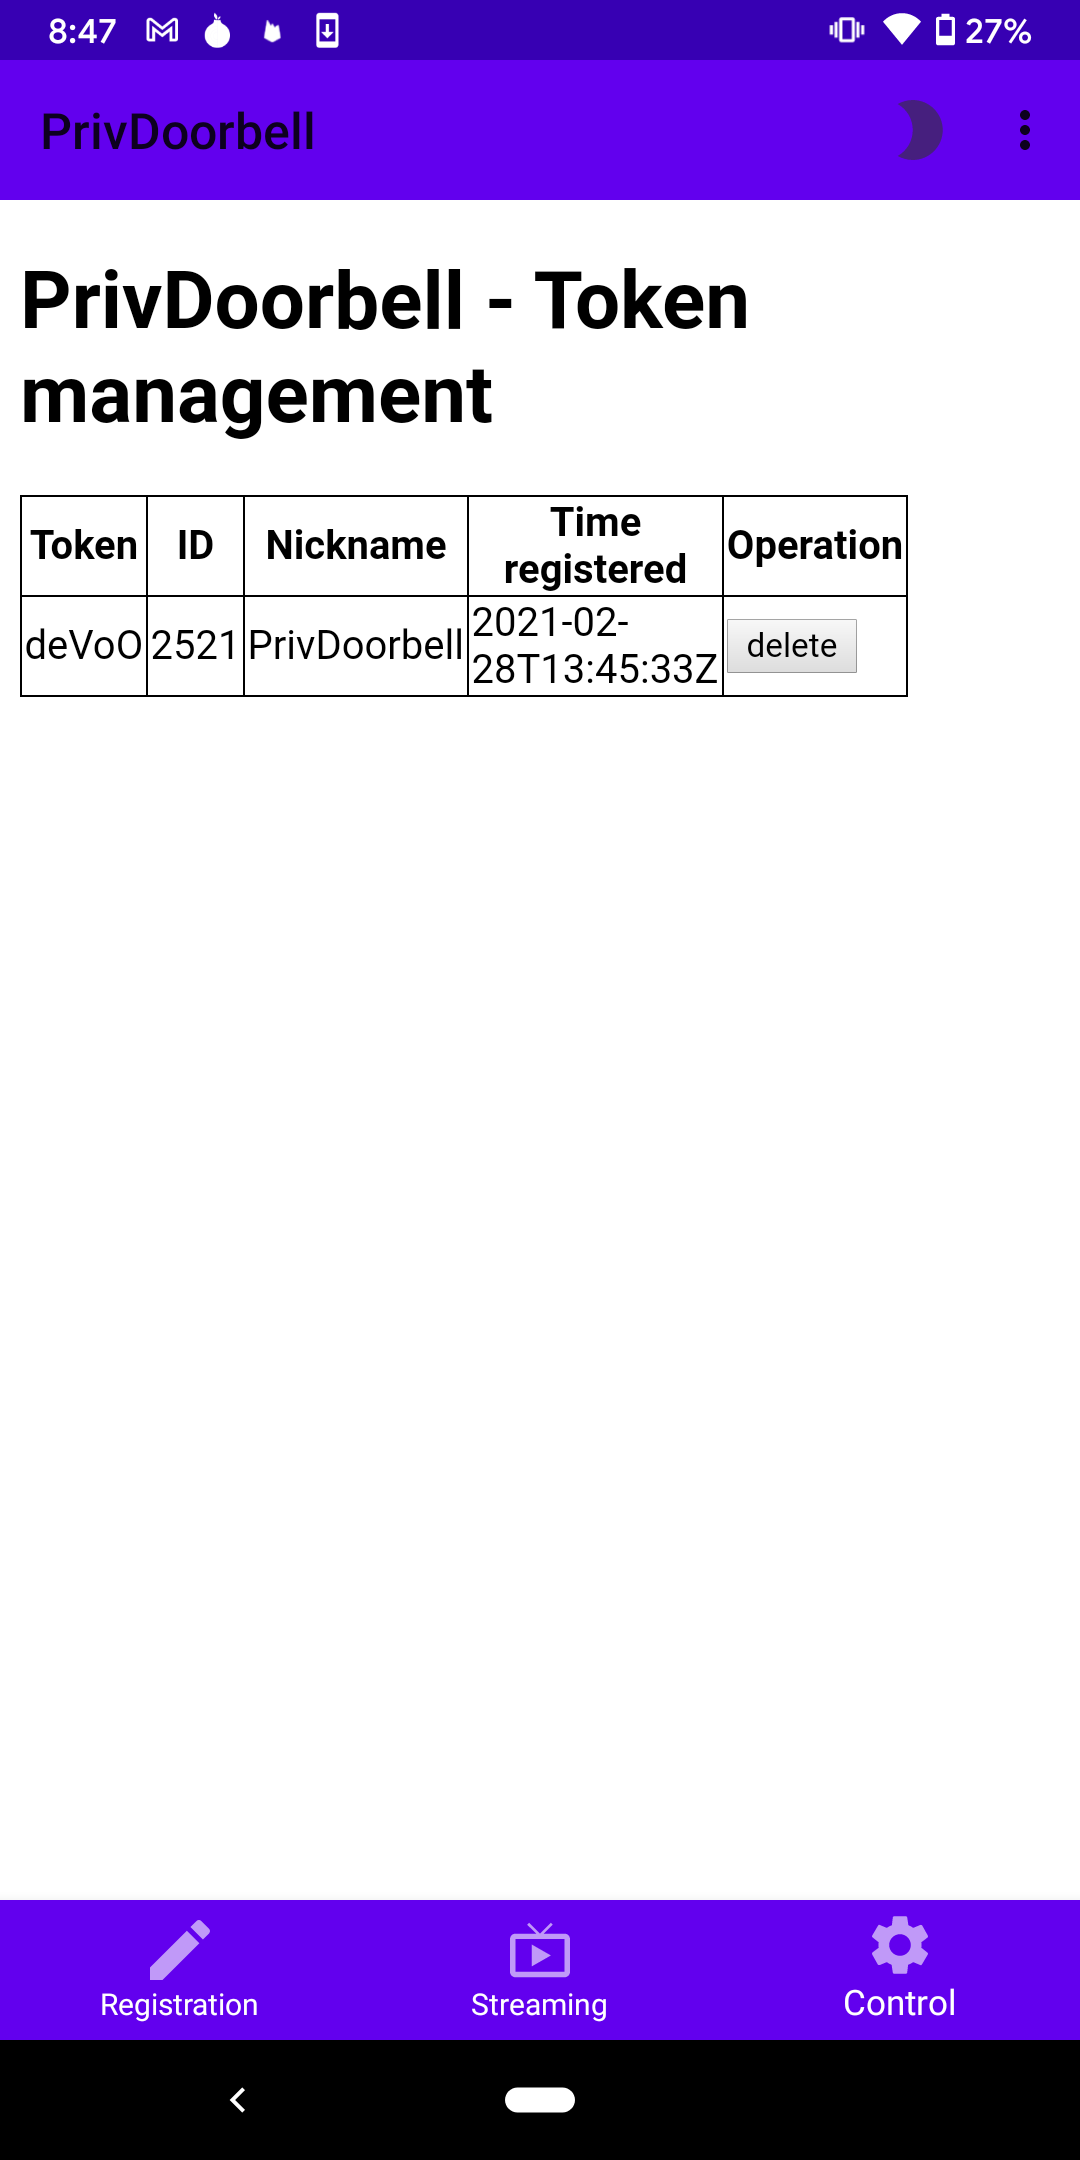
\includegraphics[width=\linewidth]{app_sc_token_revoke.png}
	\end{minipage}	
	\caption{Android app GUI examples}
	\label{fig:app_sc}
\end{figure}


\section{Performance evaluation}
In this section, we evaluate the performance of our system by analyzing the following factors:
\begin{itemize}
	\item Streaming latency
	\item Energy consumption
	\item Bandwidth
	\item Notification latency
\end{itemize}

A Google Pixel 3a XL is used as the client device.

\subsection{Streaming latency}
\label{subsec:streaming_latency}
We measure our system's latency as the time difference between the user’s pressing on the Play button and the first frame’s appearing. \textit{Fig. \ref{fig:timeconsumption}} shows the time taken for 100 samples. We divide the time into four phases.
\begin{itemize}
	\item \textbf{Circuit}. The \textit{Circuit} phase is from when the app starts processing the user’s request to when it receives the server's information. In this phase, the app queries the proxy (Orbot) about the onion URL. Orbot will then try to establish a circuit connection between the user device and the server. In practice, the time taken in this phase varies, as sometimes there is an existing circuit. If Tor has to create a new circuit, this phase typically takes a few more seconds. On average, this phase takes 2.355 seconds with a standard derivation of 3.07 seconds.
	\item \textbf{Transmission}. The \textit{Transmission} phase is from when the app sends request to the server to when the app hears back from the server. As we are using RTMP authentication, the server should return an HTTP response code 200 (indicating success) if the client provides correct credentials. The video transmission will begin immediately after the HTTP response. In average, this phase takes 0.599 seconds with a standard derivation of 0.089 seconds.
	\item \textbf{Preparation}. The \textit{Preparation} phase is from when the app receives the HTTP response from the server to when it starts filling the buffer. In this phase, the media player initializes its components and gets ready for playing the video. In average, this phase takes 3.878 seconds with a standard derivation of 0.715 seconds.
	\item \textbf{Buffering}. The \textit{Buffering} phase is when the app fills in its buffer. In this phase, the media player fill a few frames into the buffer (of a fixed size) for the decoder to decode. The decoder will decode the frames in milliseconds, and thus we can consider the video being played immediately after this phase. In average, this phase takes 0.046 seconds with a standard derivation of 0.006 seconds.
\end{itemize}

\begin{figure}
	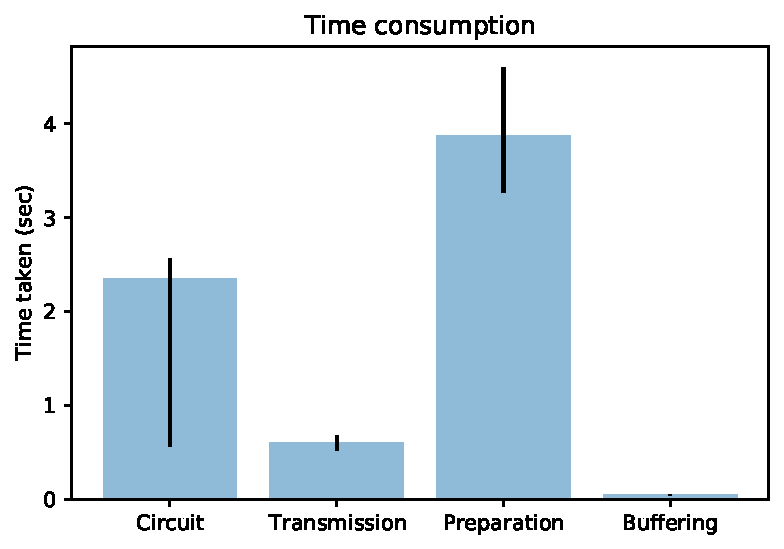
\includegraphics[width=\linewidth]{plot1.pdf}
	\caption{Time consumption of the four phases}
	\label{fig:timeconsumption}
\end{figure}

\begin{figure}
	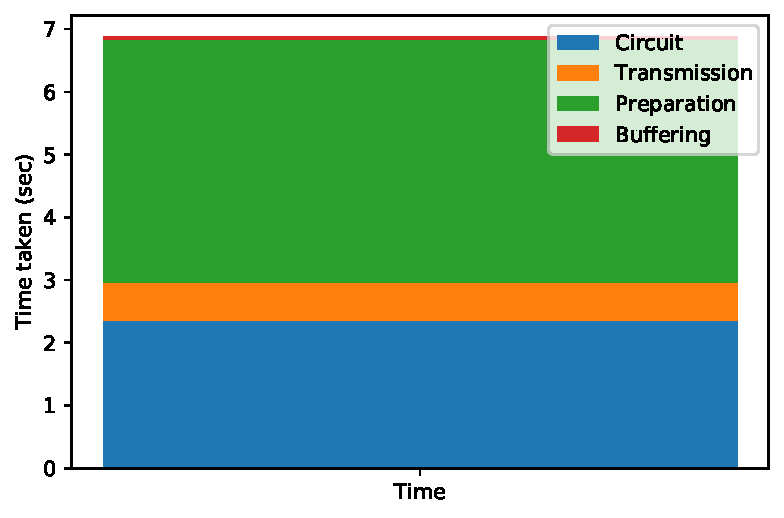
\includegraphics[width=\linewidth]{plot2.pdf}
	\caption{Time consumption of the four phases (percentage)}
	\label{fig:timepercentage}
\end{figure}

On average, the whole process takes 6.867 seconds with a standard derivation of 3.141 seconds. \textit{Fig. \ref{fig:timepercentage}} shows how much time each phase takes. While we believe a ~7 second response time is certainly noticeable, we also posit that such a delay is reasonable for our video doorbell.


\subsection{Energy consumption}
We evaluate the battery consumption of our app using the system measured data. The app consumes 6\% of the device's battery after actively running in the background for 6 days, 11 hours and 50 minutes (83.83 hours). The device has a battery size of 3700 mAh, and therefore the app roughly consumes 2.65 mAh for every hour running. We consider it reasonable for an app which receives and pushes real-time notifications.

\subsection{Bandwidth}
The outgoing traffic from the doorbell devices is 71 kb/s on average, after the video is compressed and encoded. For comparison, the raw video has an average of 410 kb/s. When not streaming the video, the doorbell's bandwidth cost is negligible.

\subsection{Video and audio quality}
The system supports videos up to 1024x768 at 6 fps and audio with a sample rate of 44.1kHz.

\subsection{Notification latency}
\label{subsec:notification_latency}
We measure the notification latency by measuring the time difference from when the message is sent to the Firebase Messaging server from the doorbell to when the message is received on the client app. The average latency of 250 consecutive samples is 0.478 seconds. Fig. \ref{fig:notificationlatency_wTor} shows the CDF (cumulative distribution function) vs. latency.

\subsection{The cost of using Tor}
Finally, we measure the cost of using Tor. By its nature, Tor adds latency to the system and we would like to know the exact impact. We measure the following time and compare the difference between:

\begin{itemize}
	\item Streaming latency
	\item Notification latency
\end{itemize}

\begin{figure}
	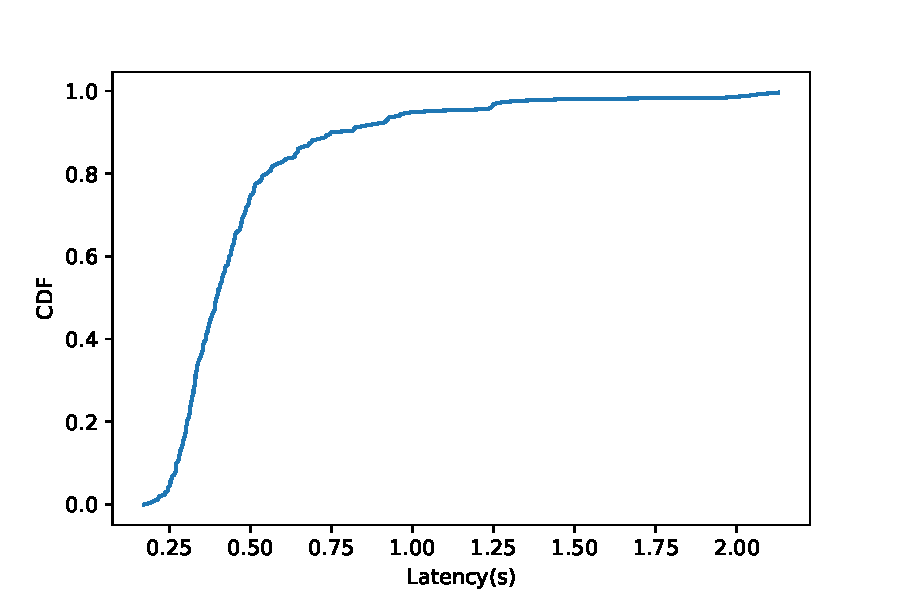
\includegraphics[width=\linewidth]{notification_latency_withTor.pdf}
	\caption{Latency of notification: with Tor}
	\label{fig:notificationlatency_wTor}
\end{figure}

\Paragraph{Streaming latency.} 

We described the streaming latency of our system in Section \ref{subsec:streaming_latency}. For a simple comparison, launching the streaming takes 2.240 seconds on average.

\Paragraph{Notification latency.}

As we described in Section \ref{subsec:notification_latency}, the latency of push notification with Tor is 0.478 seconds on average. We further conduct an experiment where Tor is not in the middle. \textit{Fig. \ref{fig:notificationlatency_wTor_vs_vanilla}} shows the difference of the service with Tor ("with-Tor") and without Tor ("vanilla"). The dotted green line denotes the latency of vanilla service, and the blue full line denotes the latency of with-Tor service. The median of with-Tor service is roughly twice the median of vanilla service.

\begin{figure}
	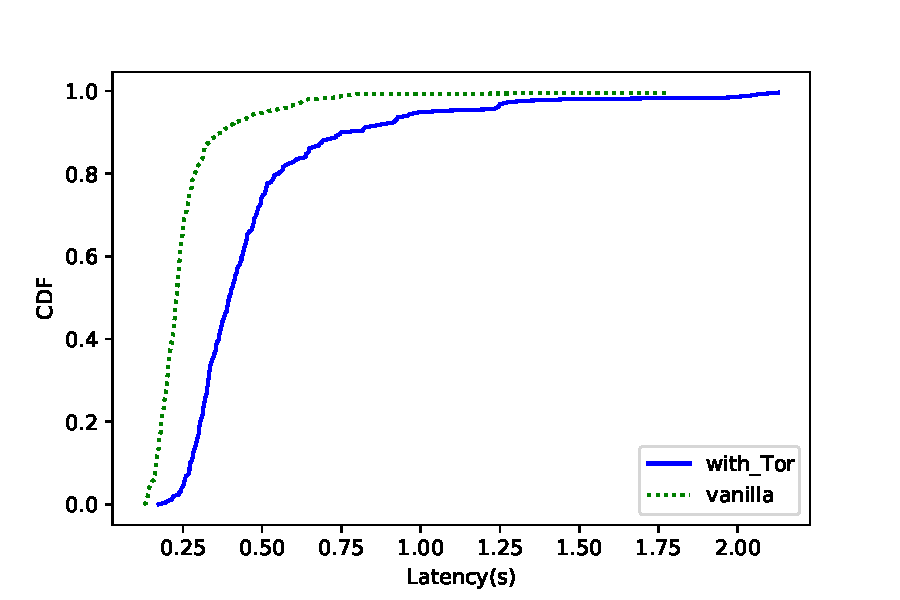
\includegraphics[width=\linewidth]{plot_push_tor_vs_vanilla.pdf}
	\caption{Latency of notification: with Tor vs. vanilla}
	\label{fig:notificationlatency_wTor_vs_vanilla}
\end{figure}